%\umlDiagram[box=,sizeX=7cm, sizeY=7cm]{
%	\umlClass[]{Deck}
%	{}
%	{
%		\umlMethod[visibility]{add}{c \emph{BasicCard}}
%		\umlMethod[visibility]{remove}{c \emph{BasicCard}}
%		\umlMethod[visibility]{remove}{i \emph{int}}
%	}
%}
\begin{figure}[h]
	\centering
	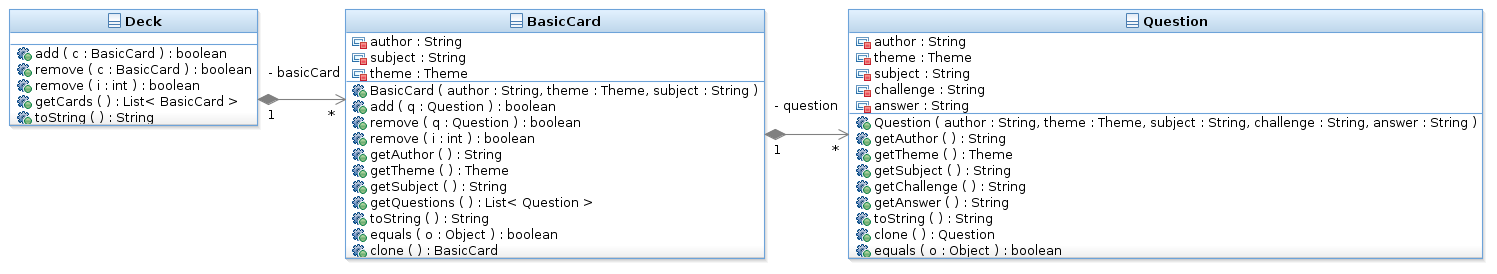
\includegraphics[width=\textwidth]{TTMC_Model_Diagram.png}
	\caption{Diagramme de classe du modèle}
	\label{fig:diag_modele}
\end{figure}

\begin{figure}[h]
	\centering
	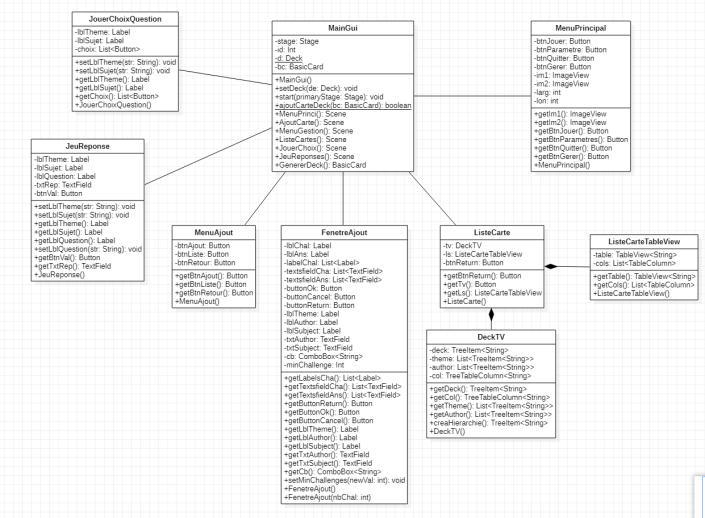
\includegraphics[width=\textwidth]{DiagrammeClasseVue.png}
	\caption{Diagramme de classe de la vue}
	\label{fig:diag_vue}
\end{figure}

Nous avons décidé de travailler avec le MainGui en position centrale. Lorsque nous changeons de scène via le click d’un bouton, nous modifions la scène via le .setScene() directement dans le MainGui. Ce qui nous permet d’avoir une répartition centralisée des modifications de scènes.
